\documentclass[12pt]{article}
\usepackage[spanish, mexico]{babel}
	%selectlanguage{spanish}
\usepackage{graphicx}
\graphicspath{{images/}}
\usepackage{amsmath}
\usepackage{wrapfig}
\usepackage{float}
\usepackage[utf8]{inputenc}

\usepackage{vmargin}
\setmarginsrb{3 cm}{2.5 cm}{3 cm}{2.5 cm}{1 cm}{1.5 cm}{1 cm}{1.5 cm}

\title{Actividad 4}
\author{Jose Pablo Salazar Velazquez}
\date{Febrero 2016}


\begin{document}

\maketitle

\section{Introducción}
En el área de la estadística, Mínimos cuadrados es una técnica de análisis numérico enmarcada dentro de la optimización matemática, en la que, dados un conjunto de pares ordenados: variable independiente, variable dependiente, y una familia de funciones, se intenta encontrar la función continua, dentro de dicha familia, que mejor se aproxime a los datos (un ``mejor ajuste''), de acuerdo con el criterio de mínimo error cuadrático 

La técnica de los mínimos cuadrados es parte de ambas secciones en el análisis de la regresión, pues se puede utilizar tanto en la regresión lineal como en el no lineal. En la actividad de hoy, se utilizaron ambos métodos para poder ajustar funciones del tipo lineal y exponencial a dos conjuntos de datos distintos con una herramienta que nos proporciona el paquete Scipy de Python.\\



\section{Actividad}
En esta practica se realizara un ajuste lineal de temperaturas medias de invierno en Nueva York y un ajuste exponencial de la presión atmosférica con respecto a la altura, utilizando los paquetes de \textit{Scipy}: \textit{curve\_fit; leastsq}.\\

\subsection{Programa 1: AjLineal.py}
En este programa se lee el documento con los datos de temperaturas medias de invierno en Nueva York, y se realiza un ajuste lineal.
\pagebreak

\subparagraph{problema 1}
\begin{verbatim}
import matplotlib.pyplot as plt 
import numpy as np

datos = np.loadtxt("lineal.txt")
x=datos[:,0]
y=datos[:,1]
print (x)
print (y)

plt.plot(x,y, 'bo')
plt.show()
\end{verbatim}
\begin{figure}[H]
	\centering
	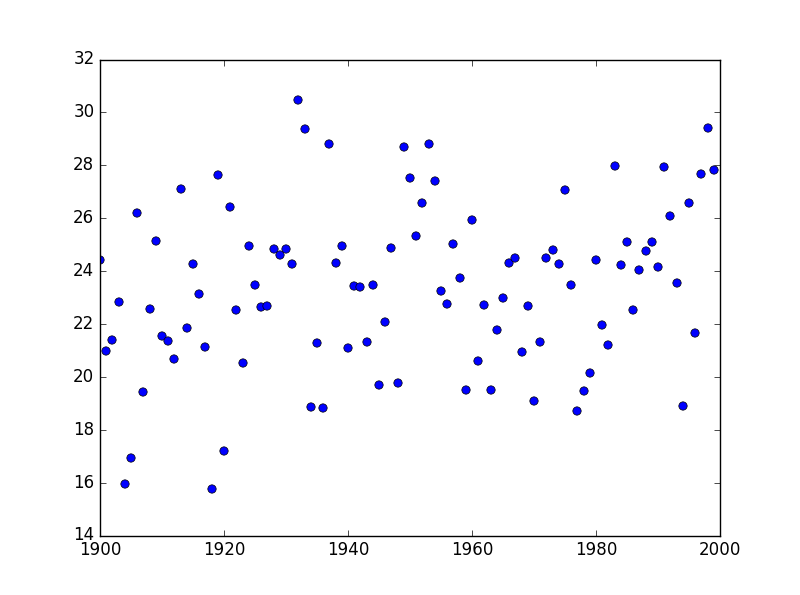
\includegraphics[width=8cm]{figure_1.png}
\end{figure}

\subsection{Programa 2}
En este programa se lee el documento con los datos de la presión atmosférica con respecto a la altura, y se realiza un ajuste exponencial.

\subparagraph{Código}
\begin{verbatim}
import numpy as np
import matplotlib.pyplot as plt
from scipy import optimize

#Leyendo el archivo con los datos
datos = np.loadtxt('lineal.txt')
x=datos[:,0]
y=datos[:,1]

print (x)
print (y)

#Escribiendo con la forma de y=mx+b
fitfunc = lambda p, x: p[0]*x + p[1]

#Distancia del punto al ajuste lineal
errfunc = lambda p, x, y: fitfunc(p, x) - y 

#Parametros patito
p0 = [1, 1] 

#Optimizando la recta
p1, success = optimize.leastsq(errfunc, p0[:], args=(x, y))

#Para la grafica
time = np.linspace(x.min(), x.max(), 100)
plt.plot(x, y, "mo", label="Data") 
plt.plot(time, fitfunc(p1, time), "g-", label="Fitted curve")

plt.title("Winter temperature in New York from 1900-1999")
plt.grid()
plt.legend()
plt.xlabel("Year")
plt.ylabel("Temperature")
\end{verbatim}
Lo que resulta de este código es lo siguiente:
\begin{figure}[H]
	\centering
	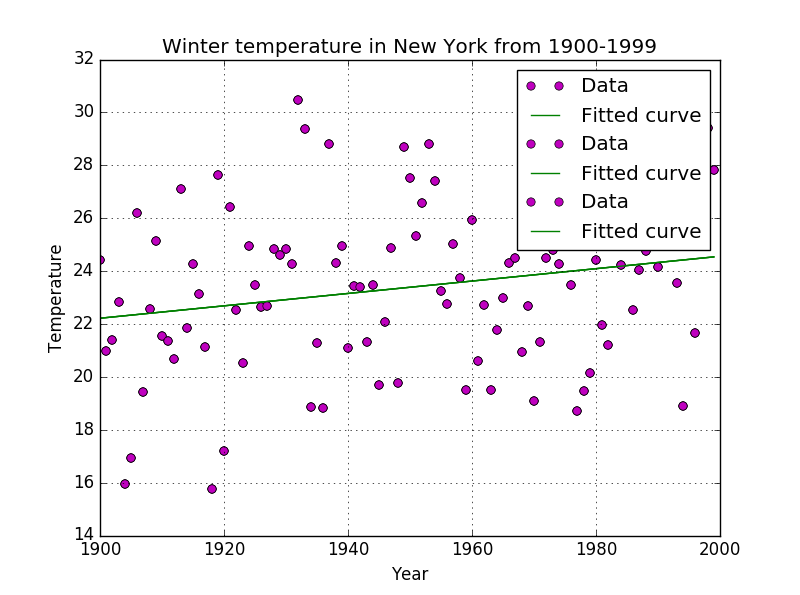
\includegraphics[width=8cm]{figure_2.png}
\end{figure}

\pagebreak

\begin{thebibliography}{3}
	
	\bibitem{Mc}
	Wikipedia,
	\emph{Mínimos cuadrados}. Recuperado de: https://es.wikipedia.org/wiki/M\% C3\% ADnimos\_cuadrados
	
	\bibitem{a}
	Lizárraga, C. (2016)
	\textit{Actividad 4 (2016-1)}. Recuperado de: http://computacional1.pbworks.com/w/page/105016164/Actividad\%204\%20(2016-1)
	

	\bibitem{Q}
	Qiku programación, (2013)
	\emph{Cómo utilizar leastsq función desde scipy.optimize en python}. Recuperado de: http://goo.gl/giZ7rO

\end{thebibliography}{3}

\end{document}